\documentclass[12pt]{article}
\setcounter{tocdepth}{4} %subsubsections in toc
\setlength{\parindent}{0pt} %no indent
\usepackage{mathtools}
\usepackage{shellesc}
\usepackage{physics}
\usepackage{esint} %for integrals
\usepackage{amssymb} %maths stuff%
\usepackage[dvipsnames]{xcolor} %for coloured text
\usepackage[hidelinks]{hyperref}
\usepackage[nameinlink, noabbrev]{cleveref}
%\usepackage[nottoc]{tocbibind}
\usepackage{tikz} %old figures package
\usepackage{pythonhighlight} % insert python code \begin{python}
\hfuzz=16pt
% \usepackage{siunitx} %for tables
\usepackage{import}
\usepackage{caption}
\usepackage{subcaption} %for subfigures
\usepackage{pstool}
\usepackage{xifthen}
\usepackage{pdfpages}
\usepackage{transparent}
\usepackage{graphicx}
\usepackage{scalefnt}
\usepackage{svg}
\usepackage{wrapfig}
\usepackage{lmodern}
\usepackage[T1]{fontenc}
\usepackage{float}

\usepackage{sectsty} % Allows customizing section commands
\allsectionsfont{\normalfont\scshape} % Make all sections centered, the default font and small caps

\usepackage{tocloft}
% Change the font for all Table of Contents entries (sections, subsections, etc.)
\renewcommand{\cfttoctitlefont}{\normalfont\scshape\Large}
\renewcommand{\cftsecfont}{\normalfont\scshape}
\renewcommand{\cftsubsecfont}{\normalfont\scshape}

% Change the font for page numbers in the Table of Contents
% \renewcommand{\cftpagefont}{\normalfont\scshape}

\usepackage{fancybox}
\usepackage{empheq}
\usepackage{tcolorbox} %Boxes for theorems and definitions
\tcbuselibrary{theorems}

\newtcbtheorem[number within=section]{mydef}{Definiton}%
{colback=SkyBlue!50,colframe=BlueViolet!80!black,fonttitle=\bfseries}{def}

\newcommand{\phantomsubsection}[1]{%
\par\refstepcounter{subsection}% Increase section counter
\sectionmark{#1}% Add section mark (header)
\addcontentsline{toc}{subsection}{\protect\numberline{\thesubsection}#1}% Add section to ToC
% Add more content here, if needed.
}

% Automatically add definitions to the ToC
\newcommand{\tocdef}[3]{%
\begin{mydef}{#1}{#2}
\phantomsubsection{#2}
#3
\end{mydef}}

\usepackage[a4paper, left=20mm, right=20mm,
top=20mm, bottom=20mm]{geometry}

%\renewcommand{\figurename}{fig} %allows custom figure numbering
\renewcommand{\tablename}{Table}

\usepackage{fancyhdr} % Custom headers and footers
\pagestyle{fancyplain} % Makes all pages in the document conform to the custom headers and footers
\fancyhead{} % No page header - if you want one, create it in the same way as the footers below

\fancyfoot[L]{} % Empty left footer
\fancyfoot[C]{} % Empty center footer
% \fancyfoot[R]{\thepage} % Page numbering for right footer
\renewcommand{\headrulewidth}{0pt} % Remove header underlines
\renewcommand{\footrulewidth}{0pt} % Remove footer underlines
\setlength{\headheight}{13.6pt} % Customize the height of the header

%
\makeatletter
\def\smallunderbrace#1{\mathop{\vtop{\m@th\ialign{##\crcr
$\hfil\displaystyle{#1}\hfil$\crcr
\noalign{\kern3\p@\nointerlineskip} %creates \smallunderbrace command
\tiny\upbracefill\crcr\noalign{\kern3\p@}}}}\limits}
\makeatother
%
\newcommand{\threebythree}[9]{
\begin{pmatrix}
{#1} & {#2} & {#3} \\
{#4} & {#5} & {#6} \\
{#7} & {#8} & {#9}
\end{pmatrix}
}

\newcommand{\twobytwo}[4]{
\begin{pmatrix}
{#1} & {#2}\\
{#3} & {#4}
\end{pmatrix}
}

\newcommand{\twobytwoasym}[1]{
\begin{pmatrix}
0 & {#1}\\
-{#1} & 0
\end{pmatrix}
}

\newcommand{\sym}[6]{
\begin{pmatrix}
{#1} & {#4} & {#5} \\
{#4} & {#2} & {#6} \\
{#5} & {#6} & {#3}
\end{pmatrix}
}

\newcommand{\antisym}[3]{
\begin{pmatrix}
0 & {#1} & {#2} \\
-{#1} & 0 & {#3} \\
-{#2} & -{#3} & 0
\end{pmatrix}
}
%
\newcommand{\ingen}{{\smash{\raisebox{0.5ex}{\scalebox{0.9}{G}}}\mkern -11mu \scalebox{1.5}{\text{I}}}}

%\setcounter{chapter}{1} % Set the chapter counter to 1
\numberwithin{equation}{subsection} % Number equations within sections (i.e. 1.1, 1.2, 2.1, 2.2 instead of 1, 2, 3, 4)
\numberwithin{figure}{subsection} % Number figures within sections (i.e. 1.1, 1.2, 2.1, 2.2 instead of 1, 2, 3, 4)
\numberwithin{table}{subsection} % Number tables within sections (i.e. 1.1, 1.2, 2.1, 2.2 instead of 1, 2, 3, 4)

%
\newcommand{\horrule}[1]{\rule{\linewidth}{#1}} % Create horizontal rule command with 1 argument of height

%\renewcommand{\bibname}{\scalefont{.7} Bibliography}

\title{%
\normalfont \normalsize
\textsc{SURE Project Notes} \\ [25pt] % Your university, school and/or department name(s)
\horrule{0.5pt} \\ [0.4cm] % Thin top horizontal rule
\huge Exoplanet Atmospheres\\ % The assignment title
\horrule{2pt} \\ [0.5cm] % Thick bottom horizontal rule
}
%
\author{O. Daniel O'Carroll\\
\small{22337259}\\
\small{\href{mailto:oocarrol@tcd.ie}{oocarrol@tcd.ie}}}
\date{\normalsize\today (45$^2$)}
\begin{document}
%\begin{minipage}{\textwidth}
\maketitle
\tableofcontents
%\end{minipage}
%
\pagebreak
%
\section{Elliptical Orbits}\label{Elliptical Orbits}
%
%
\tocdef{Kepler's Laws}{Kepler's Laws}
    {
    %
    \textbf{Kepler's First Law: Equation of Elliptical Orbits}
    \begin{empheq}[box = \shadowbox*]{align}
        r(t) = \dfrac{a(1-e^2)}{1 + e\cos(\theta(t))}.  \label{eq1.1.1}
    \end{empheq}
    %
    with $a$ being the semi-major axis $l = \dfrac{b^2}{a}$ the semi-latus rectum \\
    \textbf{Kepler's Seconds Law: Area/Angular Momentum Conservation}
    %
    \begin{empheq}[box = \shadowbox*]{align}
        A = \dfrac{1}{2m}\int_{t_0}^{t_1}J(t)dt \label{eq1.1.2}
    \end{empheq}
    %
    with $J(t) = mr^2\dot{\theta}$ a constant.\\
    \textbf{Kepler's Third Law: Orbital Period}
    %
    \begin{empheq}[box = \shadowbox*]{align}
        P^2 = \dfrac{4\pi^2}{G^2(M_\star + M_p)}a^3 \label{eq1.1.3}
    \end{empheq}
    %
    }
%
\tocdef{Lagrange Points}{Lagrange Points}
    {
    In the orbit of two bodies where one is much more massive than the other, the \textit{Lagrange points} are the points in the system which have the same orbital period as the smaller object.
    %
    \begin{figure}[H]
        \centering
        {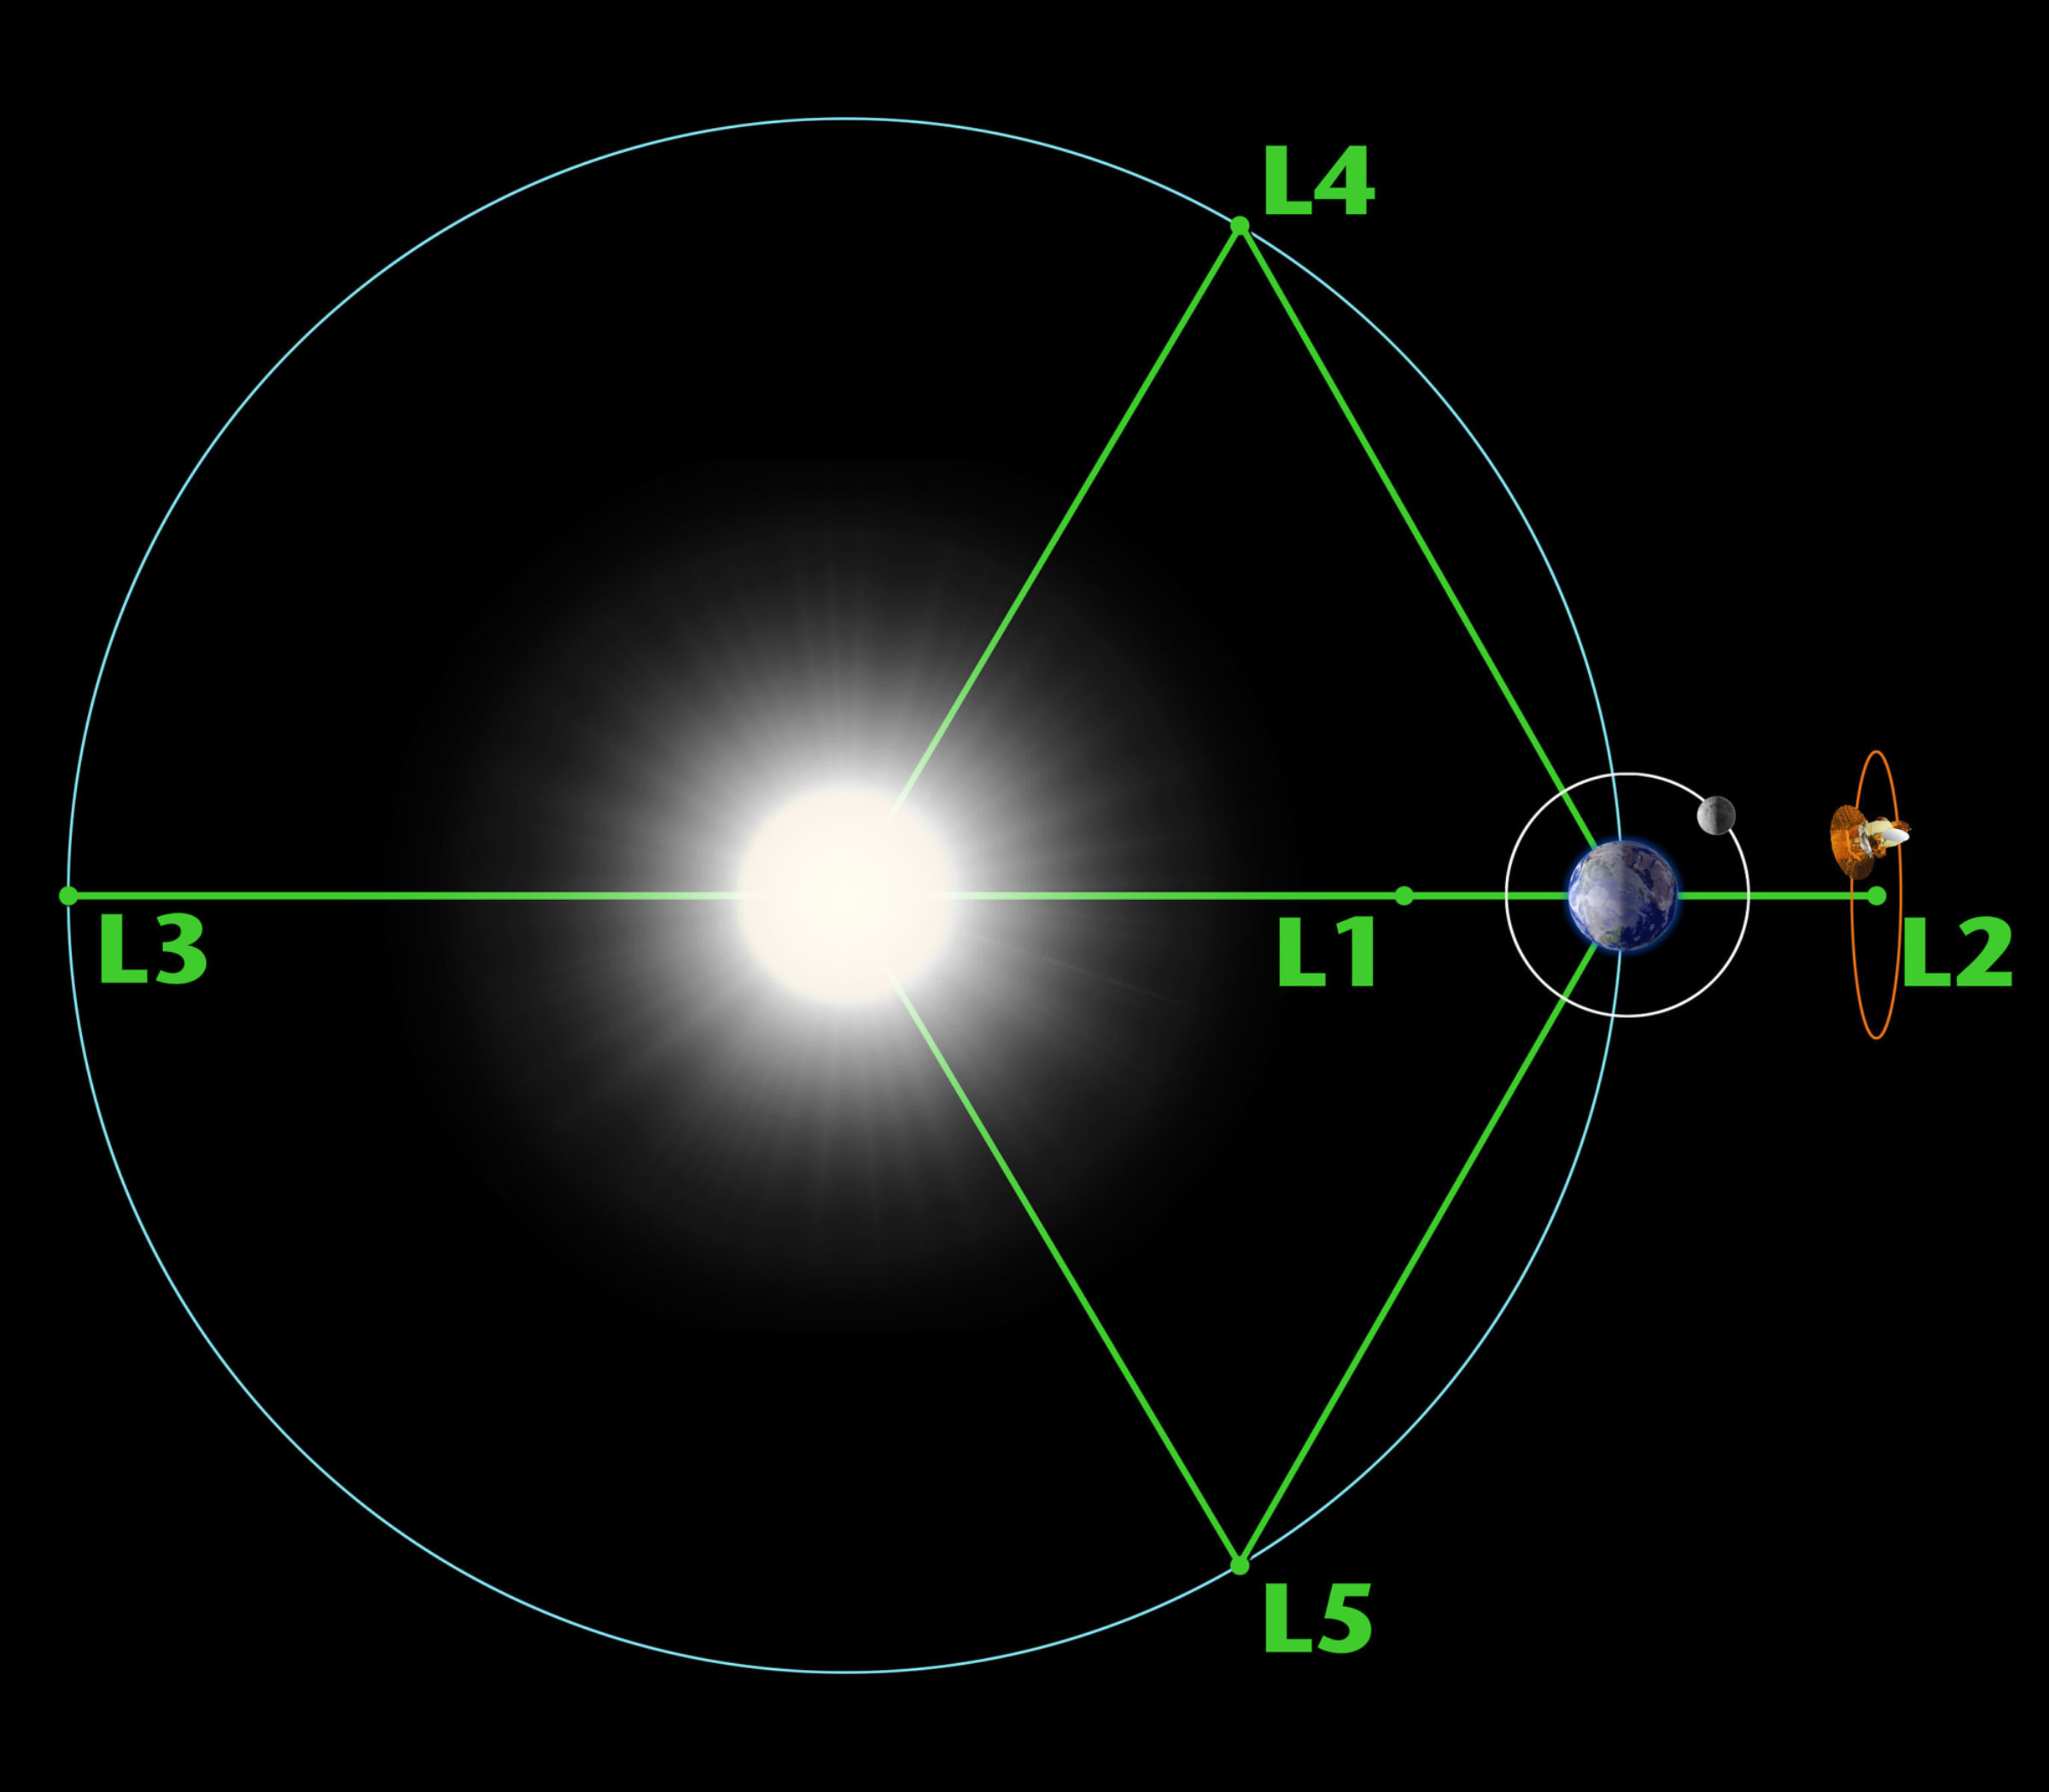
\includegraphics[width =0.5\linewidth]{lagrange_points.jpg}}
        \captionsetup{font=footnotesize}
        \caption{Diagram of the JWST in the L2 point around Earth.}
        \label{fig1.2.1}
    \end{figure}
    %
    }
%
%
\section{Keywords \& Definitions}\label{Keywords and Definitions}
%
\tocdef{Hot Jupiters}{Hot Jupiters}
    {
    Jupiter sized planet close to its host star.
    }
%
%
\tocdef{Super-Earths/Small Neptunes}{Super-Earths/Small Neptunes}
    {
    Large Earth-sized planet or small Neptune sized planet.
    }
%
%
\tocdef{Radial Velocity Semi-Amplitude}{Radial Velocity Semi-Amplitude}
    {
    %
    \begin{empheq}[box = \shadowbox*]{align}
        K = v\sin(i). \label{eq}
    \end{empheq}
    %
    }
%
%
\tocdef{Emission Spectroscopy}{Emission Spectroscopy}
    {
    Measuring the spectrum of the planets atmosphere using its own radiation.
    }
%
%
\tocdef{Transmission Spectroscopy}{Transmission Spectroscopy}
    {
    Measuring the spectrum of a planets atmosphere using the starlight of its host star when it transits.
    %
    \begin{figure}[H]
        \centering
        {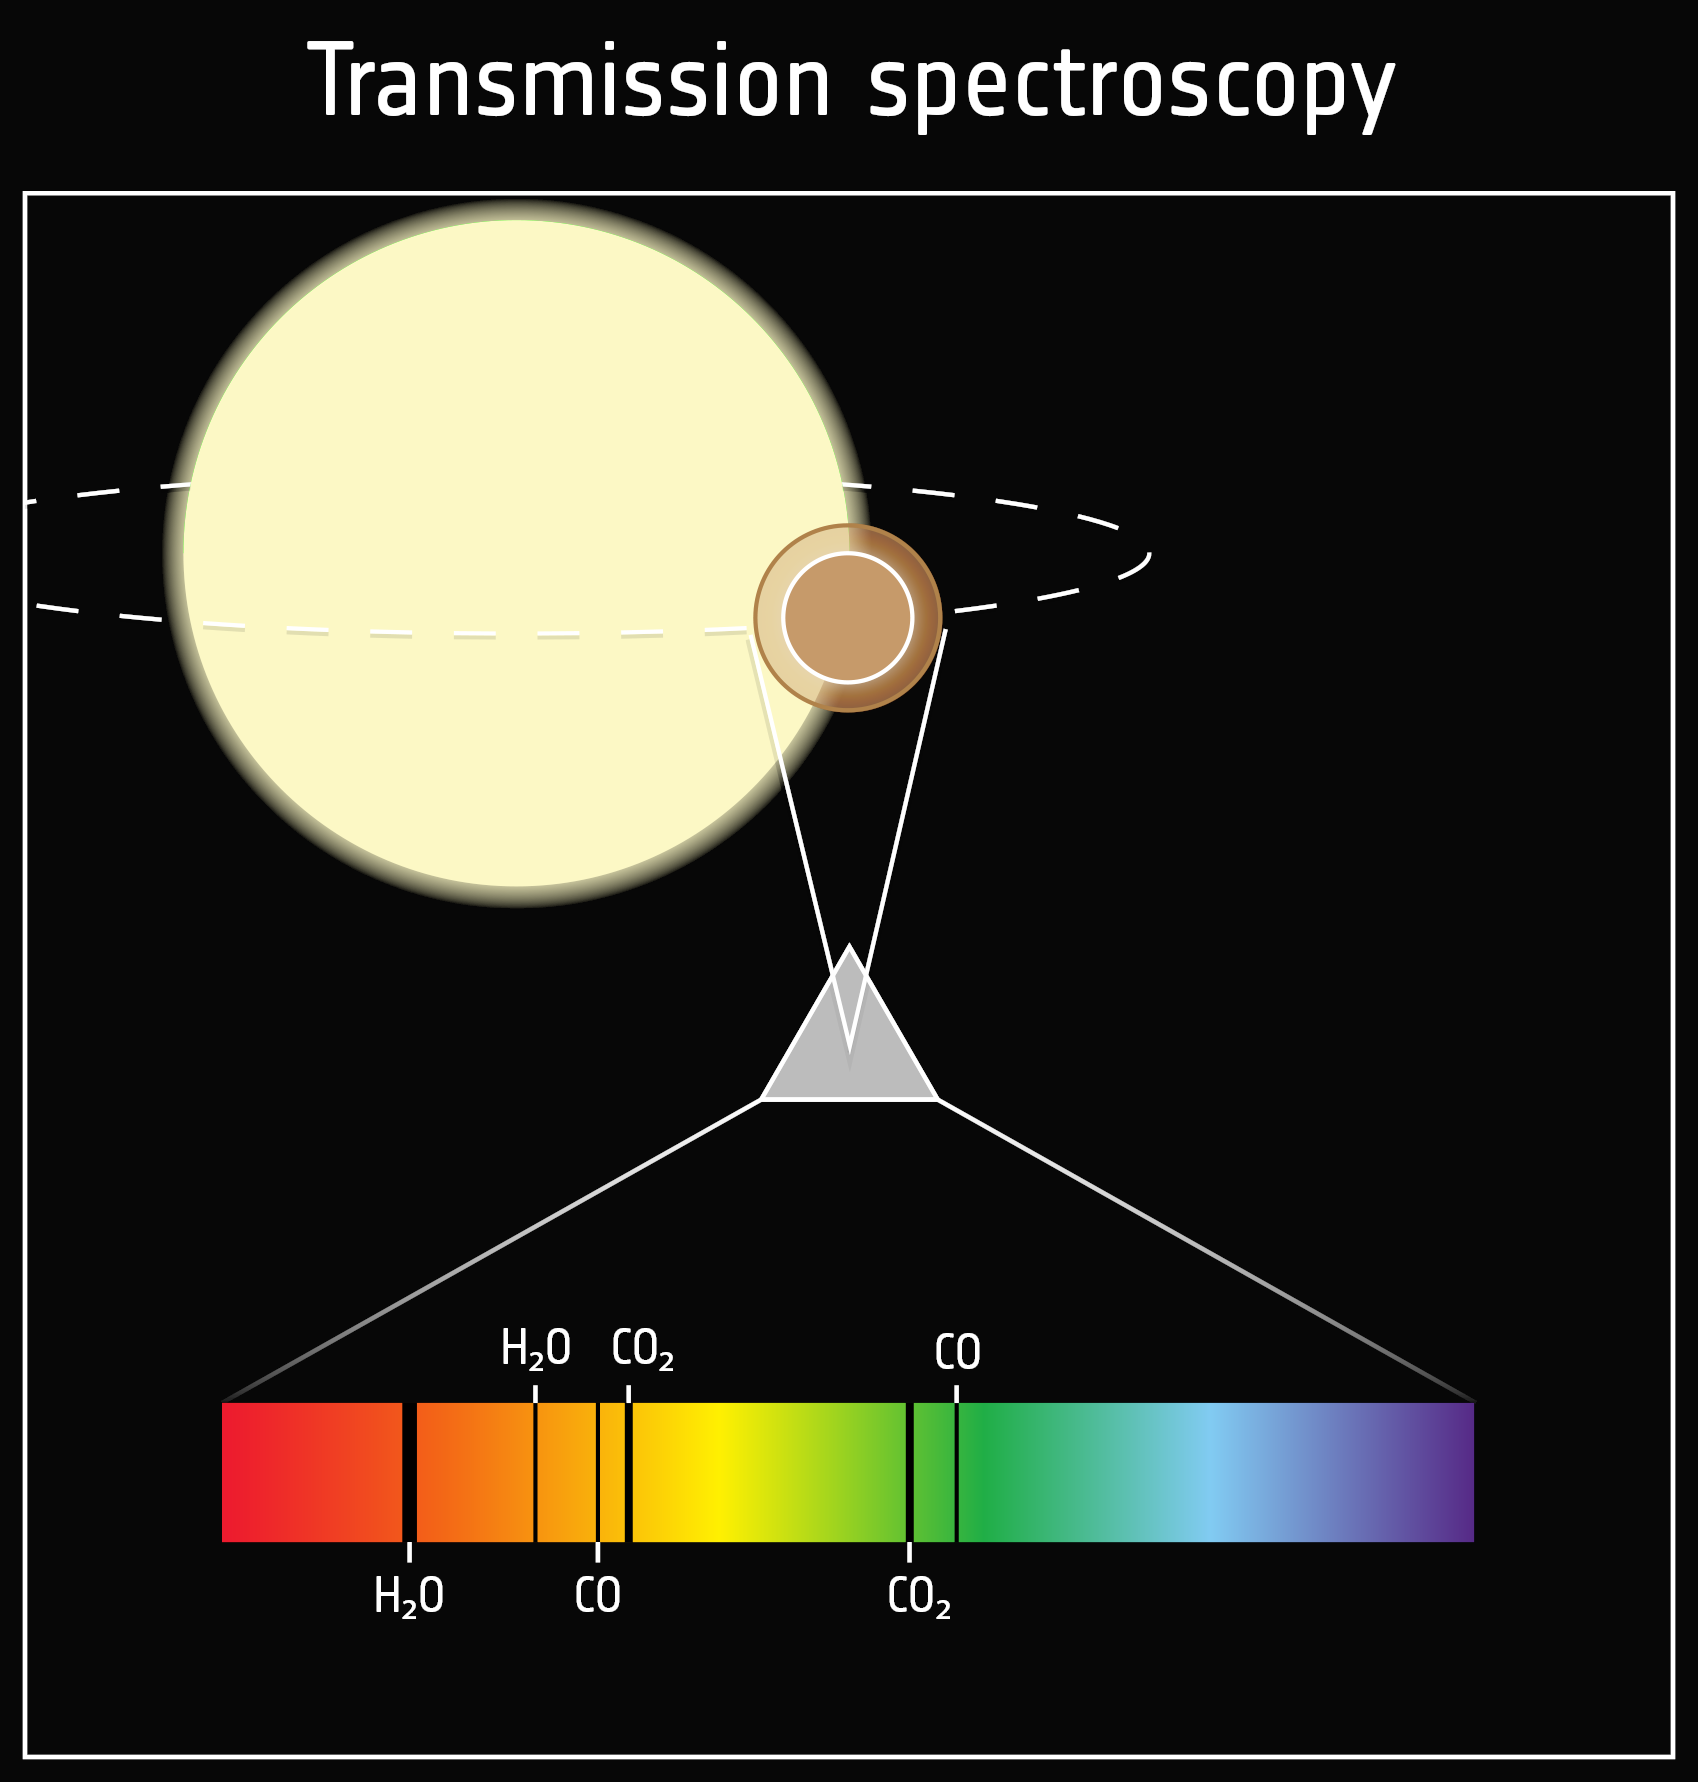
\includegraphics[width =0.5\linewidth]{Transmission_spectroscopy.png}}
        \captionsetup{font=footnotesize}
        \caption{Planet in transit and its absorbtion spectrum.}
        \label{fig2.5.1}
    \end{figure}
    %
    }
%
%
\tocdef{High vs Low Resolution Spectroscopy}{High vs Low Resolution Spectroscopy}
    {
    The formula for the resolution (or resolving power) of a spectrometer is
    %
    \begin{empheq}[box = \shadowbox*]{align}
        R = \frac{\lambda}{\Delta\lambda}. \label{eq2.6.1}
    \end{empheq}
    %
    High resolution is when $R \propto 10^6$, this is most ground-based telescopes such as the VST(Very Large Telescope). The JWST is a low resolution telescope, $R \propto 10^2$.\\

    High resolution telescopes are more complex but produce spectra with more peaks and as such are better at identifying specific molecules. They are more limited in their range as the light is diffracted more, the uncertainty in the wavelengths become larger and more importantly some of the modes start to overlap. The fix for this is to look at a narrower band of wavelengths.\\

    Low resolution spectroscopy on the other hand can have a broader band of wavelengths to detect but can't resolve individual peaks.
    }
%
%
\pagebreak
%
\section{Code and Computer Modelling}\label{Code and Computer Modelling}
%
\tocdef{Cross Correlation Functions}{Cross Correlation Functions}
    {
    When a spectrum is measured a cross correlation functions is used by taking a model of a spectrum and integrating it across the data to find the best fit.
    }
%
%
\tocdef{Kernel}{Kernel}
    {
    A kernel will be convolved with the model of the cross correlation function to account for things like the light and dark side of the planet, red and blue shifting, and atmospheric broadening.
    }
%
%
\tocdef{Retrievals}{Retrievals}
    {
    Retrievals are when the 10 or so model parameters which are statistically correlated are determined modelled and analysed, usually displayed as a 10 x 10 corner plot.}
%
%
\tocdef{petitRADTRANS Python Package}{petitRADTRANS Python Package}
    {
    Python package that can generate example spectra and create retrievals for high and low resolution spectra.
    %
    \begin{figure}[H]
        \centering
        {\includesvg[width =\linewidth]{transmission1.svg}}
        \captionsetup{font=footnotesize}
        \caption{Tutorial spectrum from petitRADTRANS \cite{3}.}
        \label{fig3.3.1}
    \end{figure}
    %
    }
%
%
\tocdef{Beer's Law}{Beer's Law}
    {
    Beer's law describes the intensity fall off due to the increase in optical path length. Below is the equation of electric flux varying with distance assuming that the light is being observed in the $x$-direction.
    %
    \begin{flalign}
        \dfrac{d \phi_e}{dx} = -\mu(x) \phi_e(x), \label{eq3.5.1}
    \end{flalign}
    %
    where $\mu(z)$ is the attenuation coefficient \cite{4}.
    }
%
%
\tocdef{Beer's Law Applied to Planetary Transits}{Beer's Law Applied to Planetary Transits}
    {
    %
    \begin{empheq}[box = \shadowbox*]{align}
    R(\lambda) = R_0 + H \left[ \gamma + \ln \left( \dfrac{P_0}{mg} \sqrt{\dfrac{2\pi R_0}{H}}\right) \right] + H\ln\sum_j\chi_j\sigma_j(\lambda),\label{eq3.6.1}
    \end{empheq}
    %
    where $H$ is the \textit{scale height}, $R_0$ is the \textit{reference radius}, $\sigma_j$ is the absorption cross-section as a function of wavelength for species $j$, $\chi_j$ is the volume mixing ratio of species $j$, $P_0$ is the pressure at the reference radius, $m$ is the mean molecular weight of the atmosphere, $g$ is the \textit{surface gravity}, and $\gamma$ is a dimensionless constant $\approx 0.56$.
    %
    \begin{empheq}[box = \shadowbox*]{align}
        H = \dfrac{kT}{mg}. \label{eq3.6.2}
    \end{empheq}
    %
    }
%
%
\pagebreak
%
\phantomsection
\addcontentsline{toc}{section}{References}
\begin{thebibliography}{999}
\bibitem{1}
\href{https://arxiv.org/abs/1001.2010}{Transits and Occultations - Joshua N Winn}
\bibitem{2}
\href{https://ui.adsabs.harvard.edu/abs/2019ARA%26A..57..617M/abstract}{Exoplanetary Atmospheres: Key Insights, Challenges, and Prospects -\\ Nikku Madhusudhan}
\bibitem{3}
\href{https://petitradtrans.readthedocs.io/en/latest/index.html}{petitRADTRANS Python package website \& documentation.}
\bibitem{4}
\href{https://academic.oup.com/mnras/article/470/3/2972/3866925}{The theory of transmission spectra revisited: a semi-analytical method for interpreting WFC3 data and an unresolved challenge -  Kevin Heng, Daniel Kitzmann}
\end{thebibliography}
\end{document}